%!TEX root = ../dynamics.tex
\section{The Evolution of Amazon MTurk From 2009 to 2014}
\label{sec:stats}

In this section, we start by describing our datasets and extract some key information and statistics that we will use in the rest of the paper.

\subsection{Crowdsourcing Platform Dataset}
\label{sec:tracker}
Over the past five years, we have periodically collected data about HITs published on \amt{}.
The data that we collect from the platform is available at \url{http://mturk-tracker.com/}. 

In this work, we consider hourly aggregated data that includes the available HIT batches and their metadata (title, description, rewards, required qualifications, etc.), in addition to their progress over time, that is, the temporal variation of the set of HITs available. In fact, one of the main metrics that we leverage (see Section \ref{sec:throughput}) is the throughput of a batch, i.e., how many HITs get completed between two successive observations. In Figure \ref{fig:motiv}, we plot the number of HITs available in a given batch versus its throughput. An interesting observation that can be made is that large batches can achieve high throughput (thousands of HITs per minute).

In total, our dataset covers more than 2.5M different batches with over 130M HITs.
We note that the tracker reports data periodically only and does not reflect fine-grained information (e.g., variations at each second). We believe however that it captures enough information to perform meaningful, long-term trend analyses and to understand the dynamics and interactions within the crowdsourcing platform.\\

\begin{figure}[tb]
	\centering
		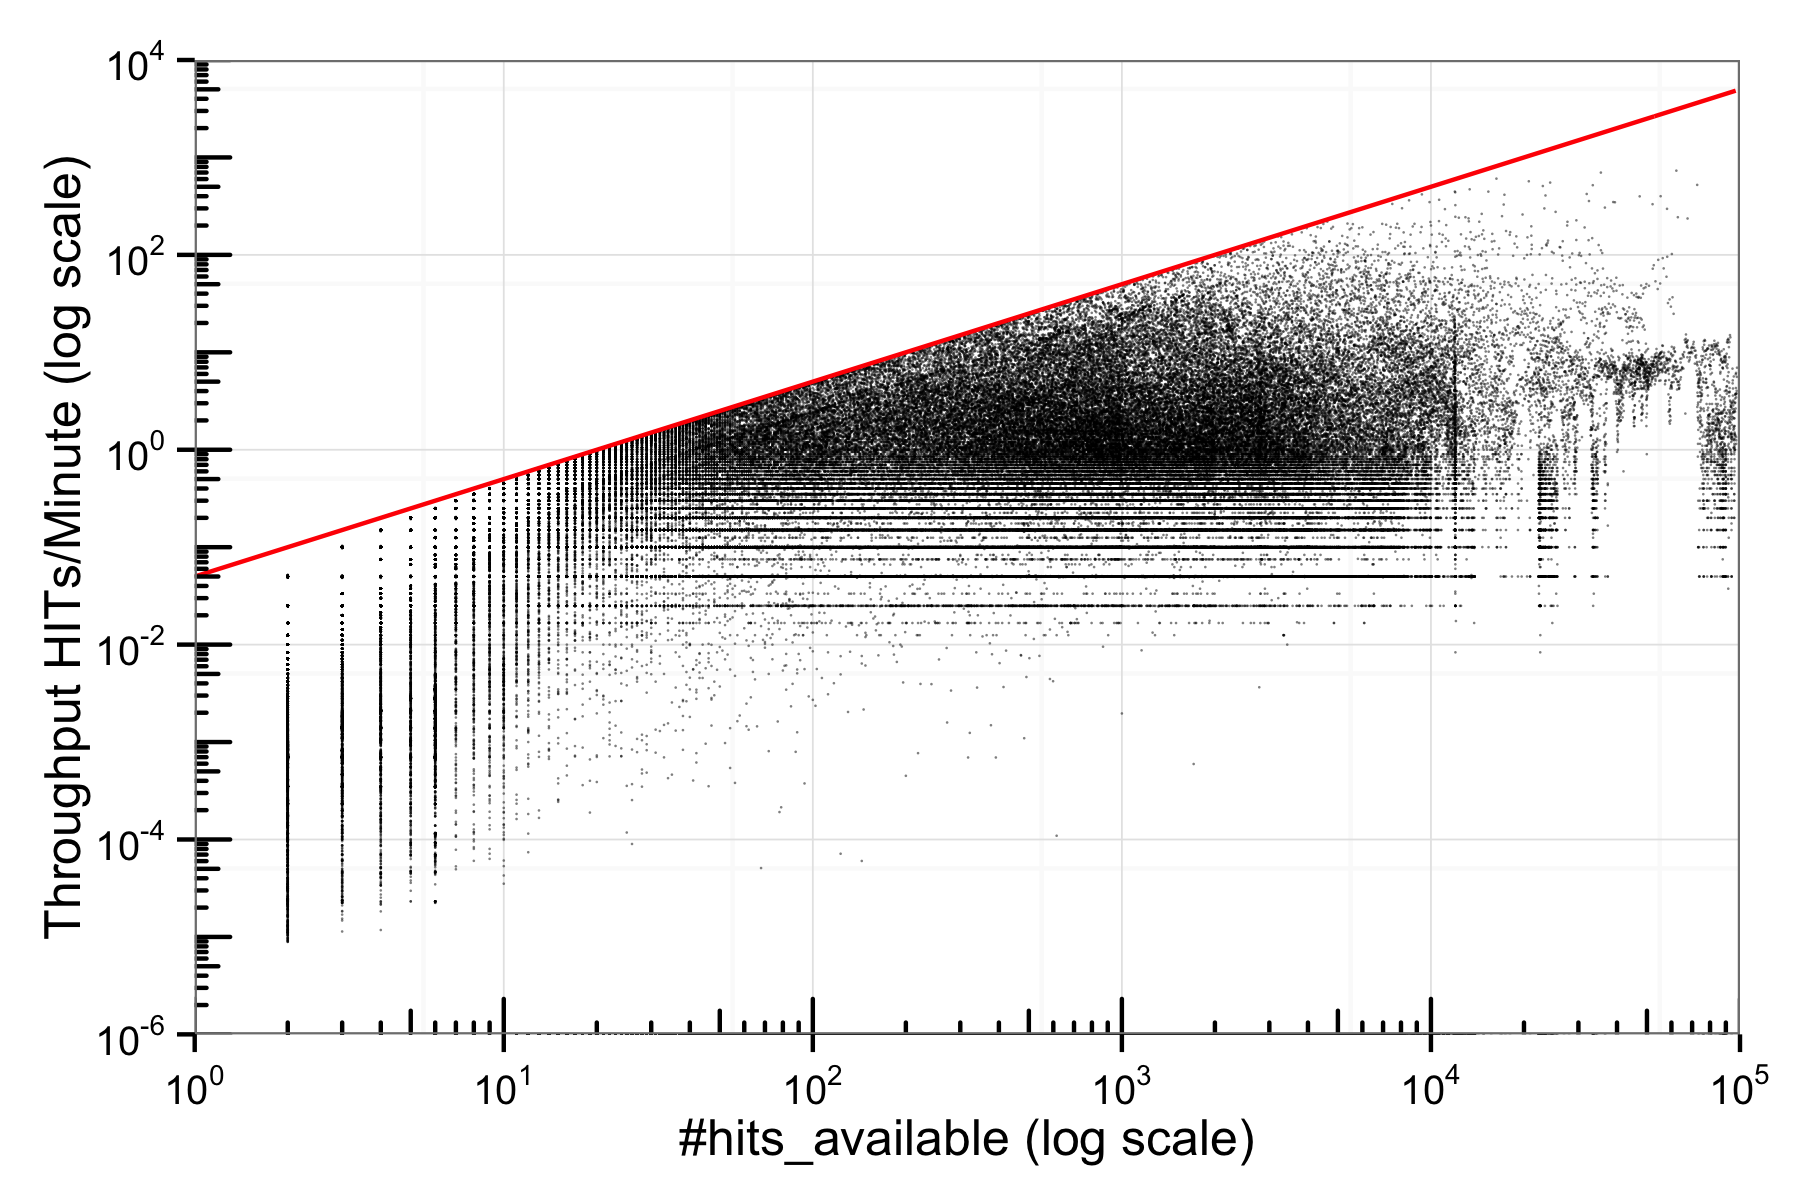
\includegraphics[width=0.48\textwidth]{figures/motiv_mturk}
	\caption{Batch throughput versus number of HITs available in the batch. The red line corresponds to the maximum throughput we could have observed due to the tracker periodicity constraints. For readability, this graph represents a subset of 3 months (January-March 2014).}
	\label{fig:motiv}
\end{figure}
\begin{figure}[tb]
	\centering
		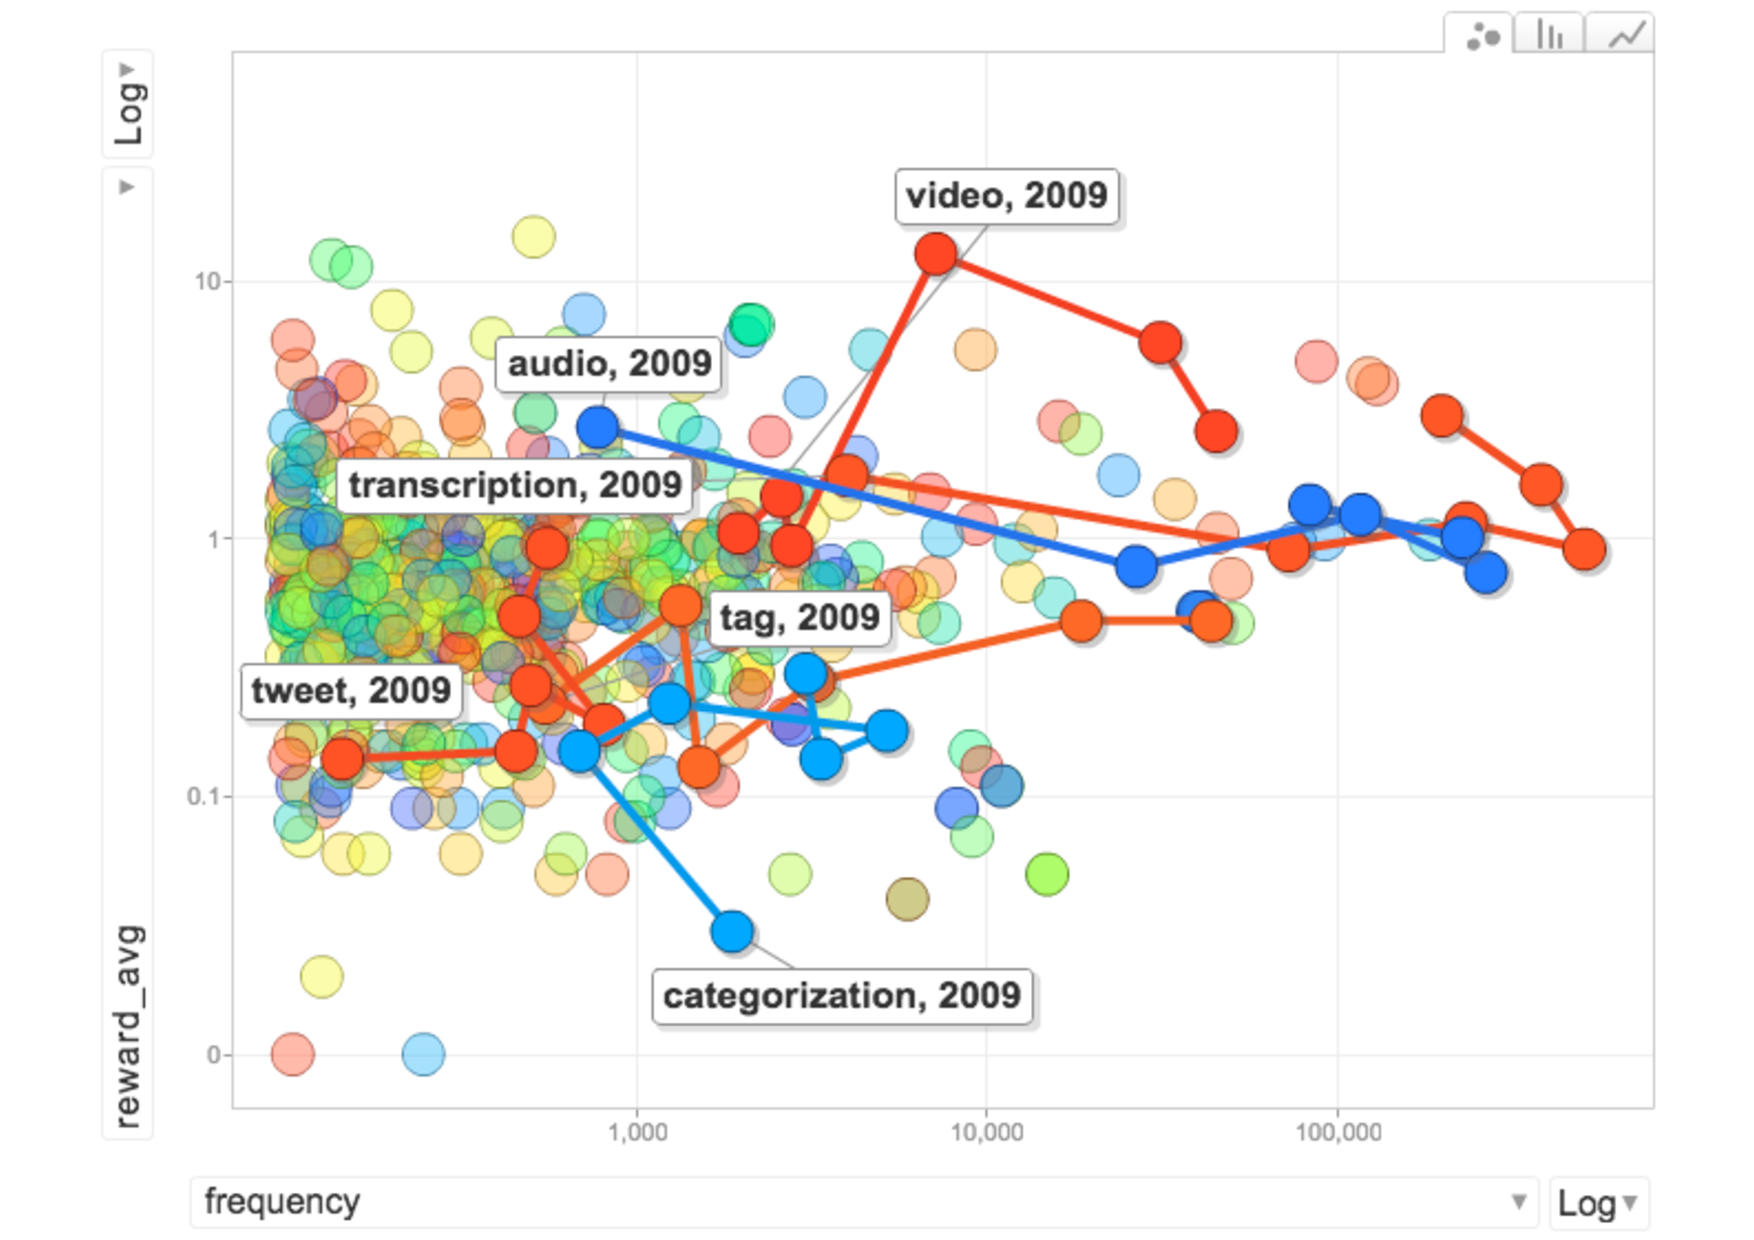
\includegraphics[width=0.45\textwidth]{figures/tagEvolution}
	\caption{The use of keywords to annotate HITs. $frequency$ corresponds to how many times a keyword was used, and $reward\_avg$ corresponds to the average monetary reward of batches that listed the keyword.}
	\label{fig:tagEvolution}
\end{figure}
\begin{figure*}[tb]
	\centering
		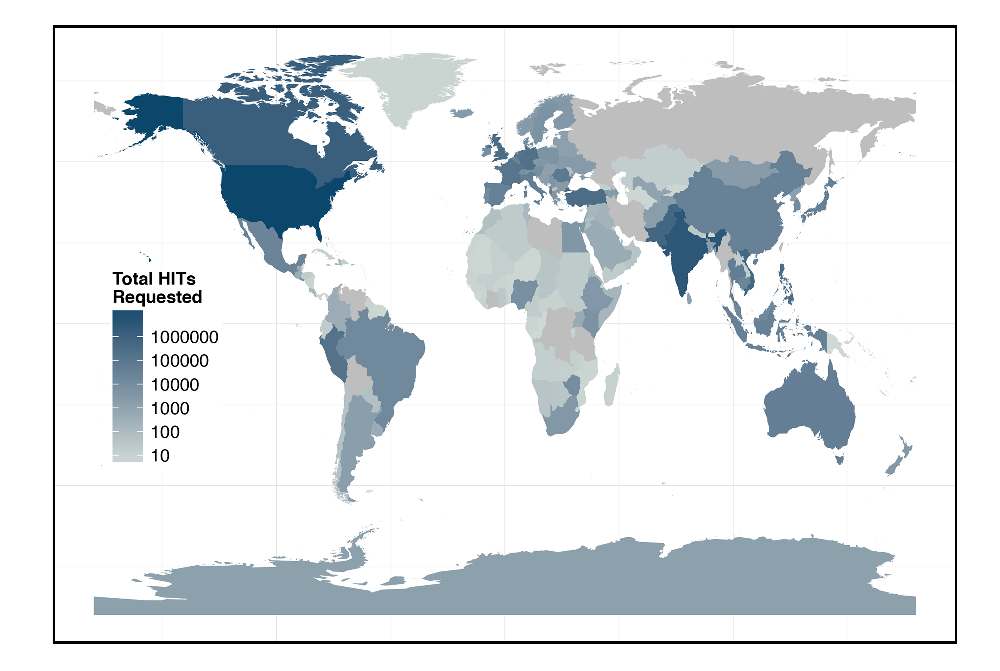
\includegraphics[width=0.5\textwidth]{figures/map}
		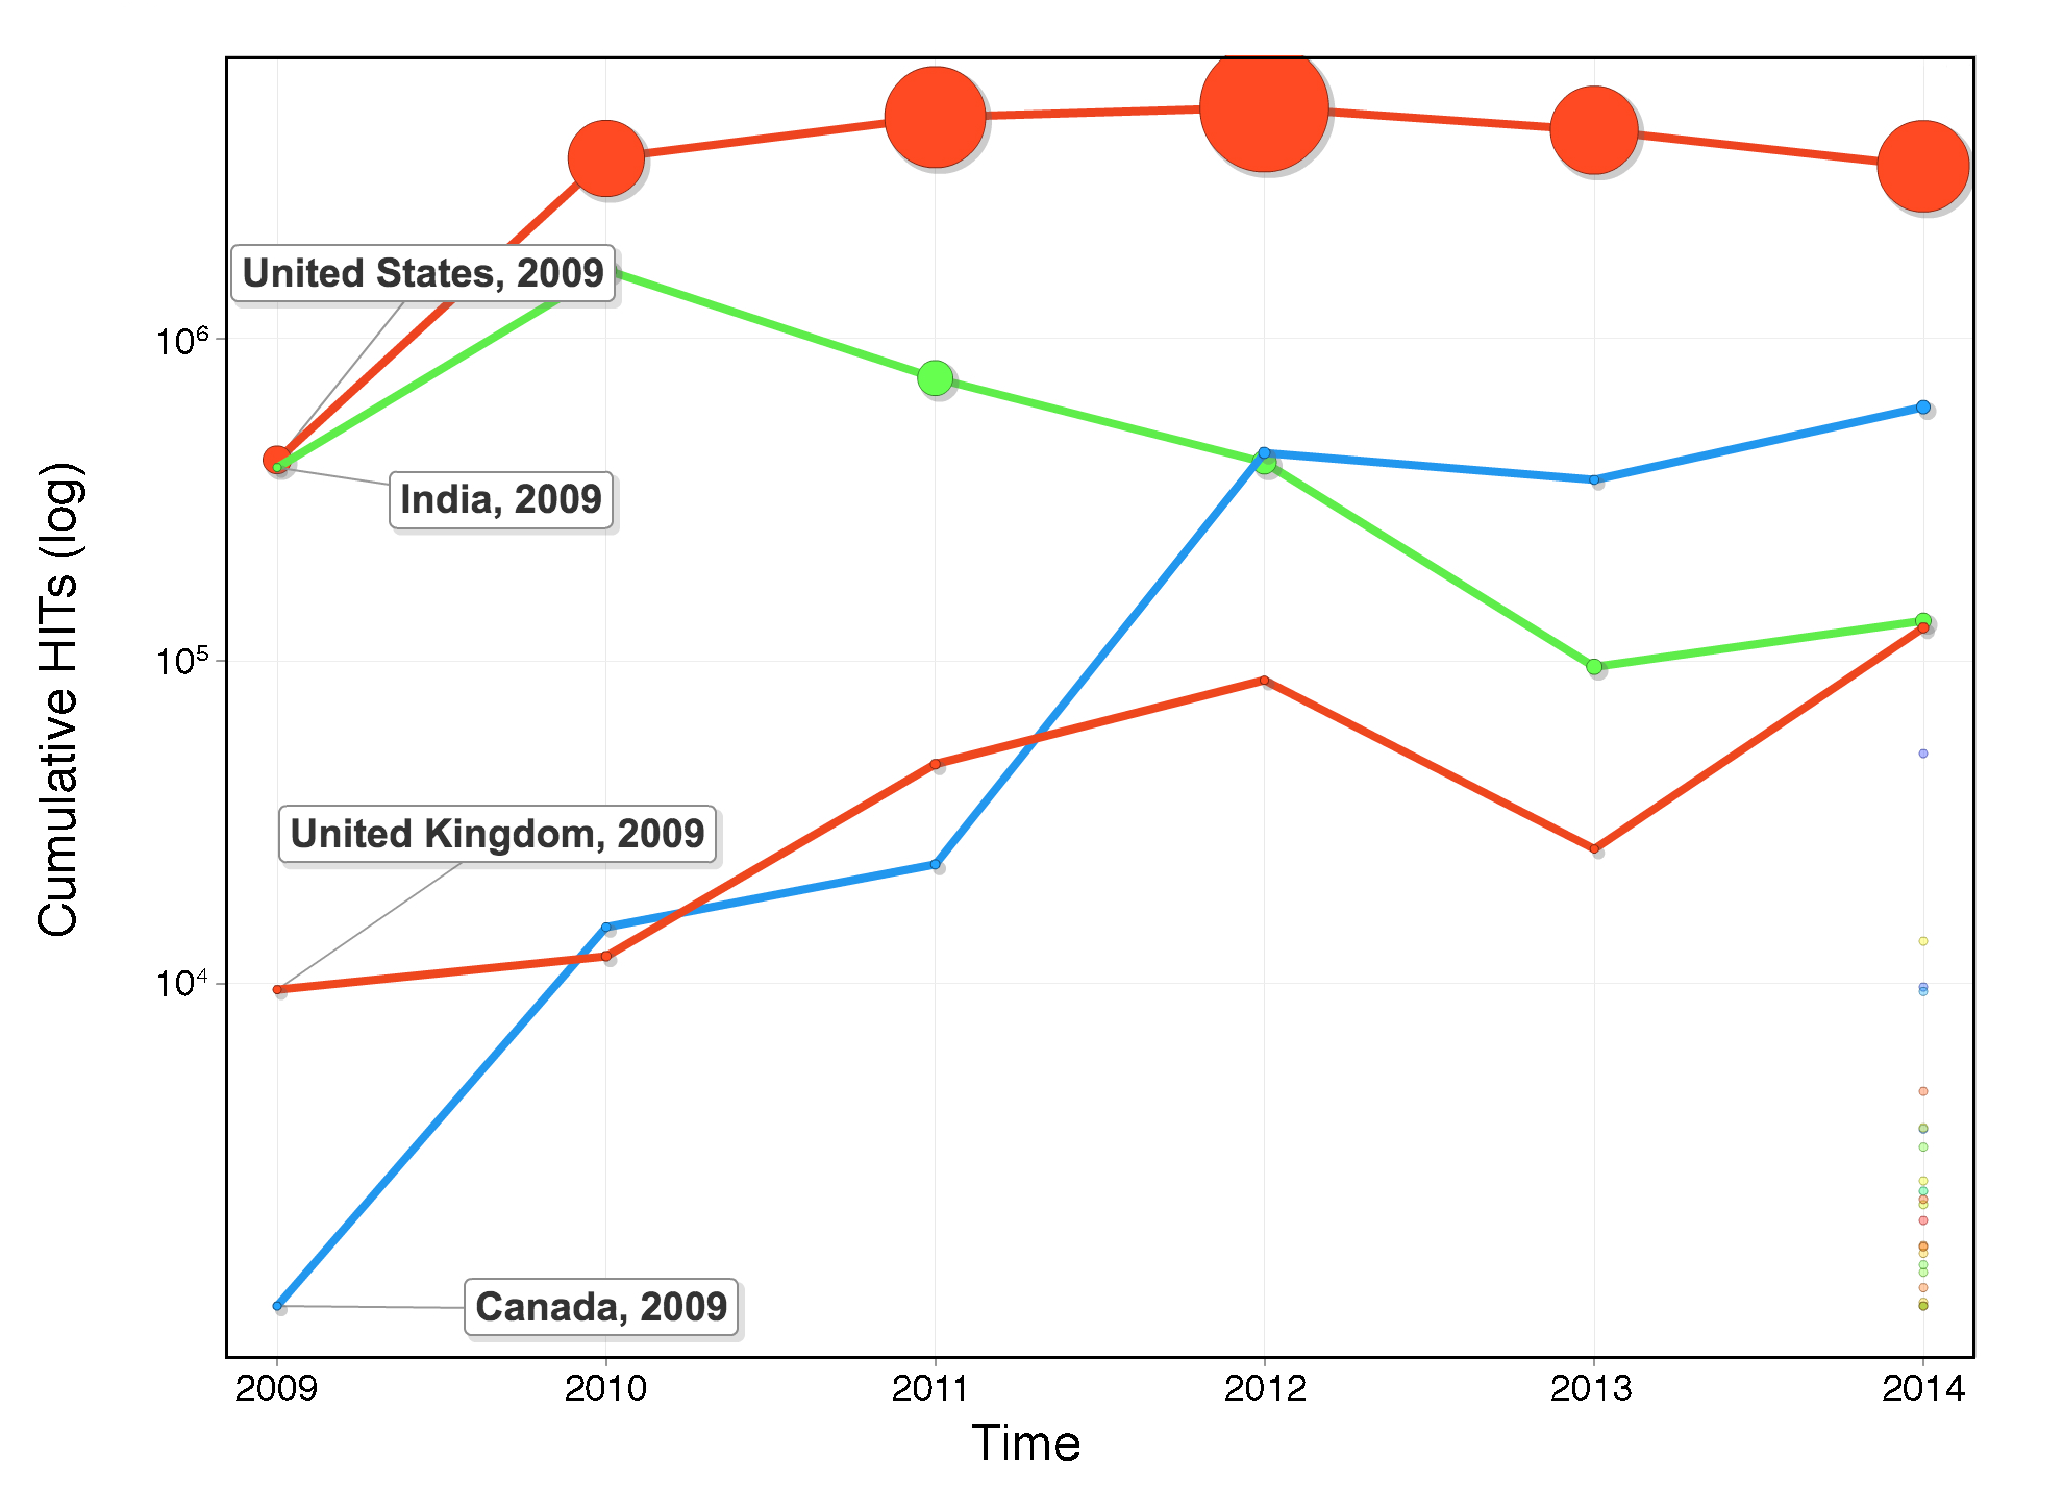
\includegraphics[width=0.40\textwidth]{figures/countriesTime}
	\caption{HITs with specific country requirements. On the left-hand side, the countries with the most HITs dedicated to them. On the right-hand side, the time evolution (x-axis) of country-specific HITs with volume (y-axis) and reward (size of data point) information.}
	\label{fig:country}
\end{figure*}

\subsection{A Data-driven Analysis of Platform Evolution}
First, we identify trends obtained from aggregated information over time, keywords, and countries associated to the published HITs.  Each of the following analyses is also available as an interactive visualization over the historical data on \url{http://xi-lab.github.io/mturk-mrkt/}.
\paragraph{Topics  Over Time}
First we want to understand how different topics have been addressed by means of micro-task crowdsourcing over time.
In order to run this analysis, we look at the keywords associated with published HITs. We observe the evolution of keyword popularity and associated reward on \amt{}. 
%plot explanation
Figure \ref{fig:tagEvolution} shows this behavior. Each point in the plot represents a keyword associated to the HITs with its frequency (i.e., number of HITs with this keyword) on the x-axis, and the average reward in a given year on the y-axis. The path connecting data points indicates the time evolution, starting in 2009, with one point representing the keyword usage over one year.

% observations
We observe that the frequency of the `audio' and `transcription' keywords (i.e., blue and red paths from left to right) have substantially increased over time. They have become the most popular keywords in the last two years and are paid more than \$1 on average.
HITs with the `video' tag have also increased in number with a reward that has reached a peak in 2012 and decreased after that.
HITs tagged as `categorization' have been paid consistently in the range of \$0.10-\$0.30 on average, except in 2009 where they were rewarded less than \$0.10 each.
HITs tagged as `tweet' have not increased in number but have been paid more over the years, reaching \$0.9 on average in 2014: This can be explained by more complex tasks being offered to workers, such as sentiment classification or writing tweets.

\paragraph{Preferred Countries by Requesters Over Time}
Figure \ref{fig:country} shows the requirements set by requesters with respect to the countries they wish to select workers from. The left part of Figure \ref{fig:country} shows that most HITs are to be completed exclusively by workers located in the US, India, or Canada. The right part of Figure \ref{fig:country} shows the evolution over time of the country requirement phenomenon.
The plot shows the number of HITs with a certain country requirement (on the y-axis) and its time evolution (on the x-axis) with yearly steps. The size of the data points indicates the total reward associated to those HITs.

We observe that US-only HITs dominate, both in terms of their sheer number as well as in terms of the reward associated to them. 
Interestingly, we notice how HITs for workers based in India have been decreasing over time. %This can be explained by \amt{} restrictions on accepting new workers outside of the US on the platform.
On the other hand, HITs for workers based in Canada have been increasing over time, becoming in 2014 larger than those exclusively available to workers based in India.  We also see that the reward associated to them is smaller than the budget for India-only HITs.
As of 2014, both HITs for workers based in Canada or UK are more numerous that those for workers based in India.
Overall, 88.5\% of the HIT batches that were posted in the considered time period did not require any specific worker location. 86\% of those which did imposed a constraint requesting US-based workers.


Figure \ref{fig:keyword_loc} shows the top keywords attached to HITs restricted to specific locations.
\begin{figure}[tb]
	\centering
		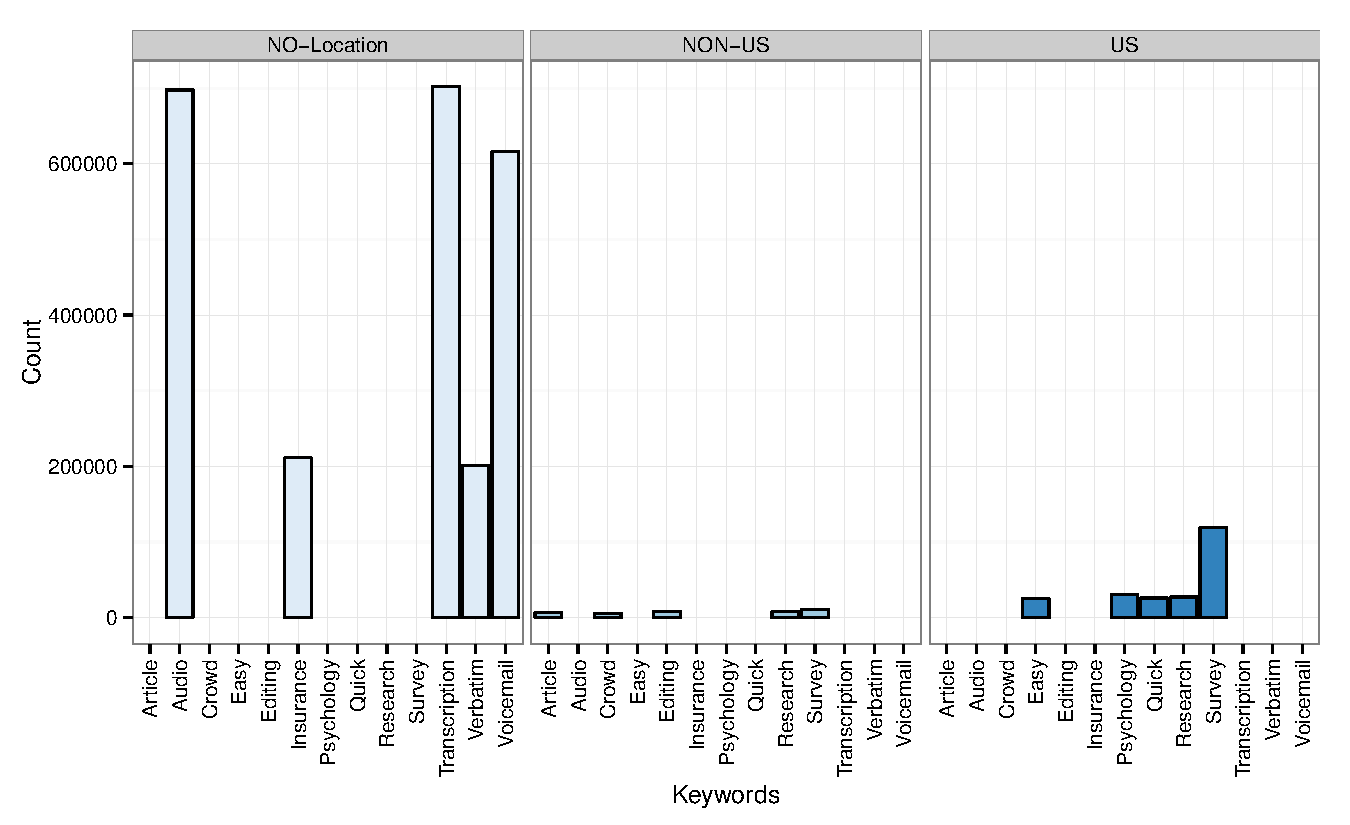
\includegraphics[width=0.5\textwidth]{figures/keywords_location}
	\caption{Keywords for HITs restricted to specific countries.}
	\label{fig:keyword_loc}
\end{figure}
We observe that the most popular keywords (i.e., `audio' and `transcription') do not require country-specific workers. 
%This suggests that restricting workers from a single country for large batches would make their completion much slower. 
We also note that US-only HITs are most commonly tagged with `survey'.

% \subsection{Why Did Certain Requesters Quit?}
% \subsection{Does reputation Improve Throughput?}

\paragraph{HIT Reward Analysis}
Figure \ref{fig:reward_year} shows the most frequent rewards assigned to HITs over time\footnote{Data for 2014 has been omitted as it is not comparable with other year values.}. We observe that while in 2011 the most popular reward was \$0.01, recently HITs paid \$0.05 are getting more frequent. This can be explained both by how workers search for HITs on \amt{} and by the \amt{} fee scheme. Requesters now prefer to publish more complex HITs possibly with multiple questions in them and grant a higher reward: This also attracts those workers who are not willing to complete a HIT for small rewards and reduces the fees paid to \amt{}, which are computed based on the number of HITs published on the platform.

\begin{figure}[tb]
	\centering
		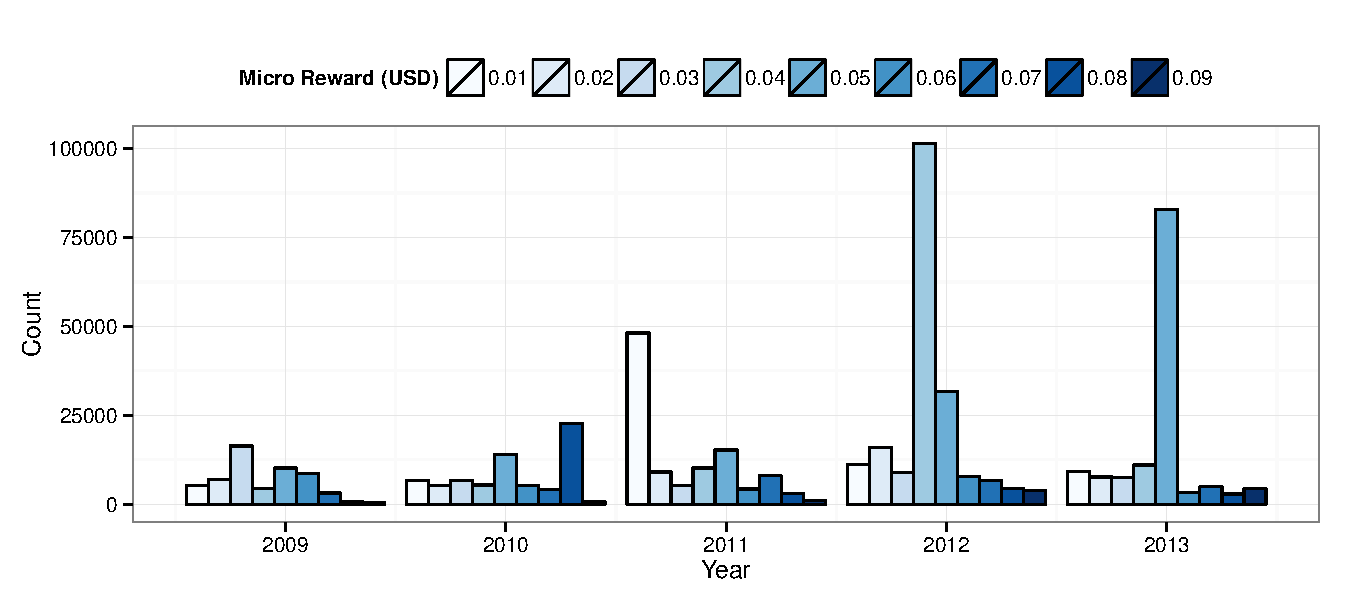
\includegraphics[width=0.5\textwidth]{figures/reward_year}
	\caption{Popularity of HIT reward values over time.}
	\label{fig:reward_year}
\end{figure}



\paragraph{Requester Analysis}
In order to be sustainable, a crowdsourcing platform needs to retain requesters over time or get new requesters to replace those who do not publish HITs anymore. Figure \ref{fig:requesters_reward} shows the number of new requesters who used \amt{} and the overall number of active requesters at a certain point in time. We can observe an increasing number of active requesters over time and a constant number of new requesters who join the platform (at a rate of 1,000/month over the last two years).

\begin{figure}[tb]
	\centering
		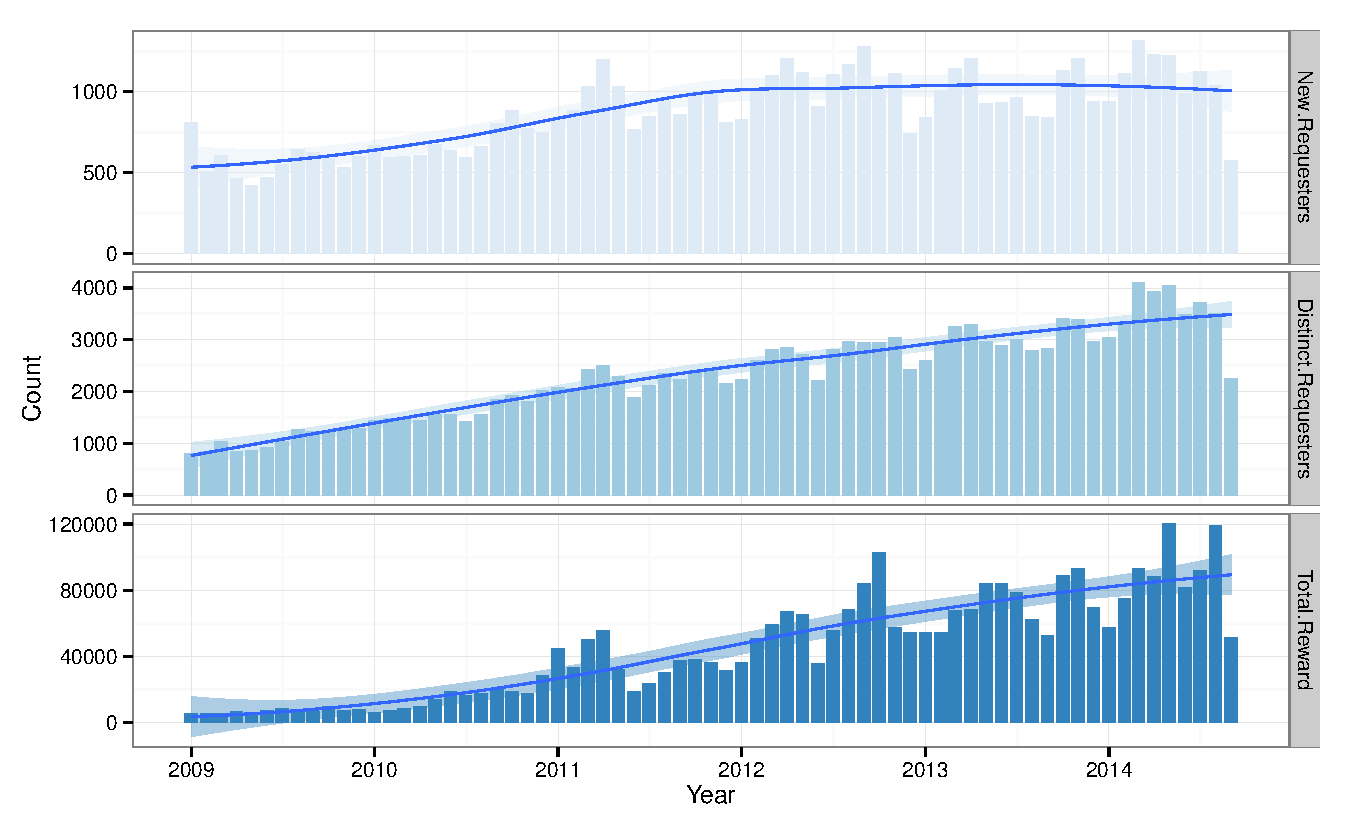
\includegraphics[width=0.5\textwidth]{figures/requesters_reward}
	\caption{Requester activity and total reward on the platform over time. The line over the data shows local polynomial regression fitting \cite{cleveland1992local}.}
	\label{fig:requesters_reward}
\end{figure}

It is also interesting to look at the overall amount of reward for HITs published on the platform, as platform revenues are computed as a function of HIT reward. From the bottom part of Figure \ref{fig:requesters_reward}, we observe a linear increase in the total reward for HITs on the platform. Interestingly, we also observe some seasonality effects over the years, with October being the month with the highest total reward and January or February being the month with minimum total reward.


\paragraph{HIT Batch Size Analysis}
When a lot of data needs to be crowdsourced (e.g., when many images needs to be tagged), multiple  tasks containing similar HITs can be published together. We define a batch of HITs as a set of similar HITs published by a requester at a certain point in time. 

Figure \ref{fig:batch_size_pow} shows the distribution of batch sizes in the period from 2009 to 2014. We can observe that most of the batches were of size 1 (more than 1M), followed by a long tail of larger, but less frequent, batch sizes.

Figure \ref{fig:batch_size} shows how batch size has changed over time. We observe that the average batch size have slightly decreased. The monthly median is 1 (due to the heavily skewed distribution). Another observation that can be made is that in 2014 very large batches containing more that 200,000 HITs have appeared on \amt{}.

\begin{figure}[tb]
	\centering
		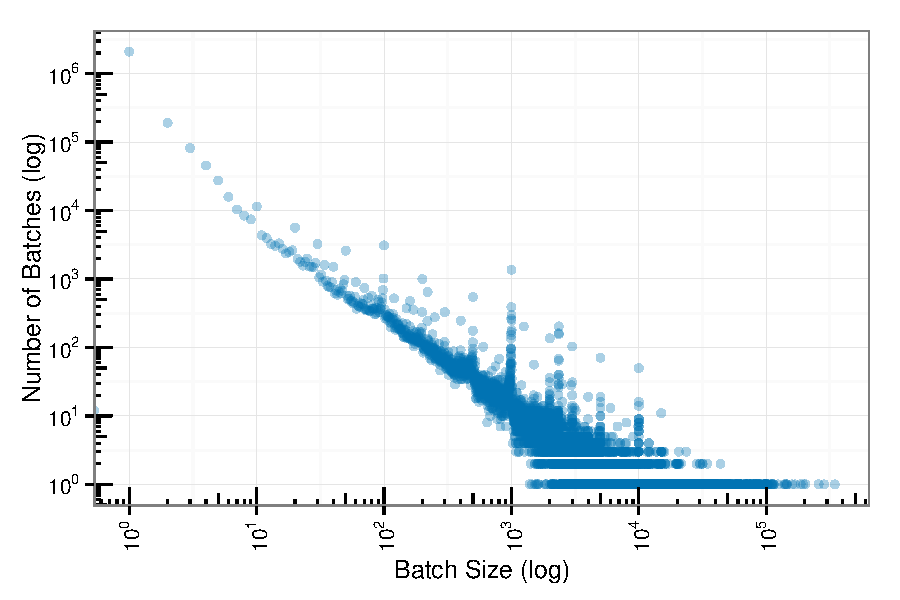
\includegraphics[width=0.5\textwidth]{figures/powerlaw}
	\caption{The distribution of batch sizes.}
	\label{fig:batch_size_pow}
\end{figure}

\begin{figure}[tb]
	\centering
		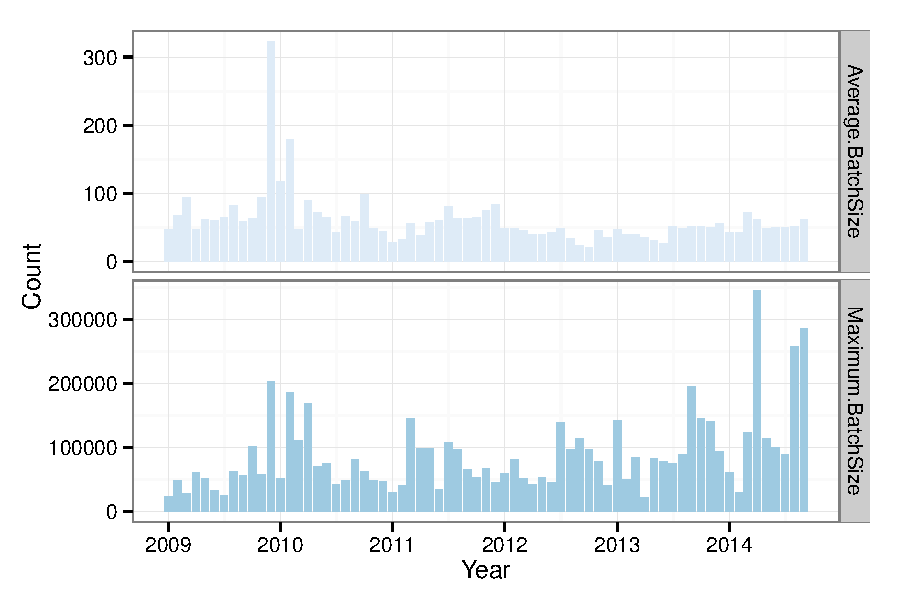
\includegraphics[width=0.5\textwidth]{figures/batch_size}
	\caption{Batch Sizes. The line over the data shows local polynomial regression fitting \cite{cleveland1992local}.}
	\label{fig:batch_size}
\end{figure}


